\section{Plan and Schedule}\label{sec:timeplan}
The time schedule, mentioned below, is only provisional and might change
during development process by {$\pm$}10\% of the total time.

\begin{center}
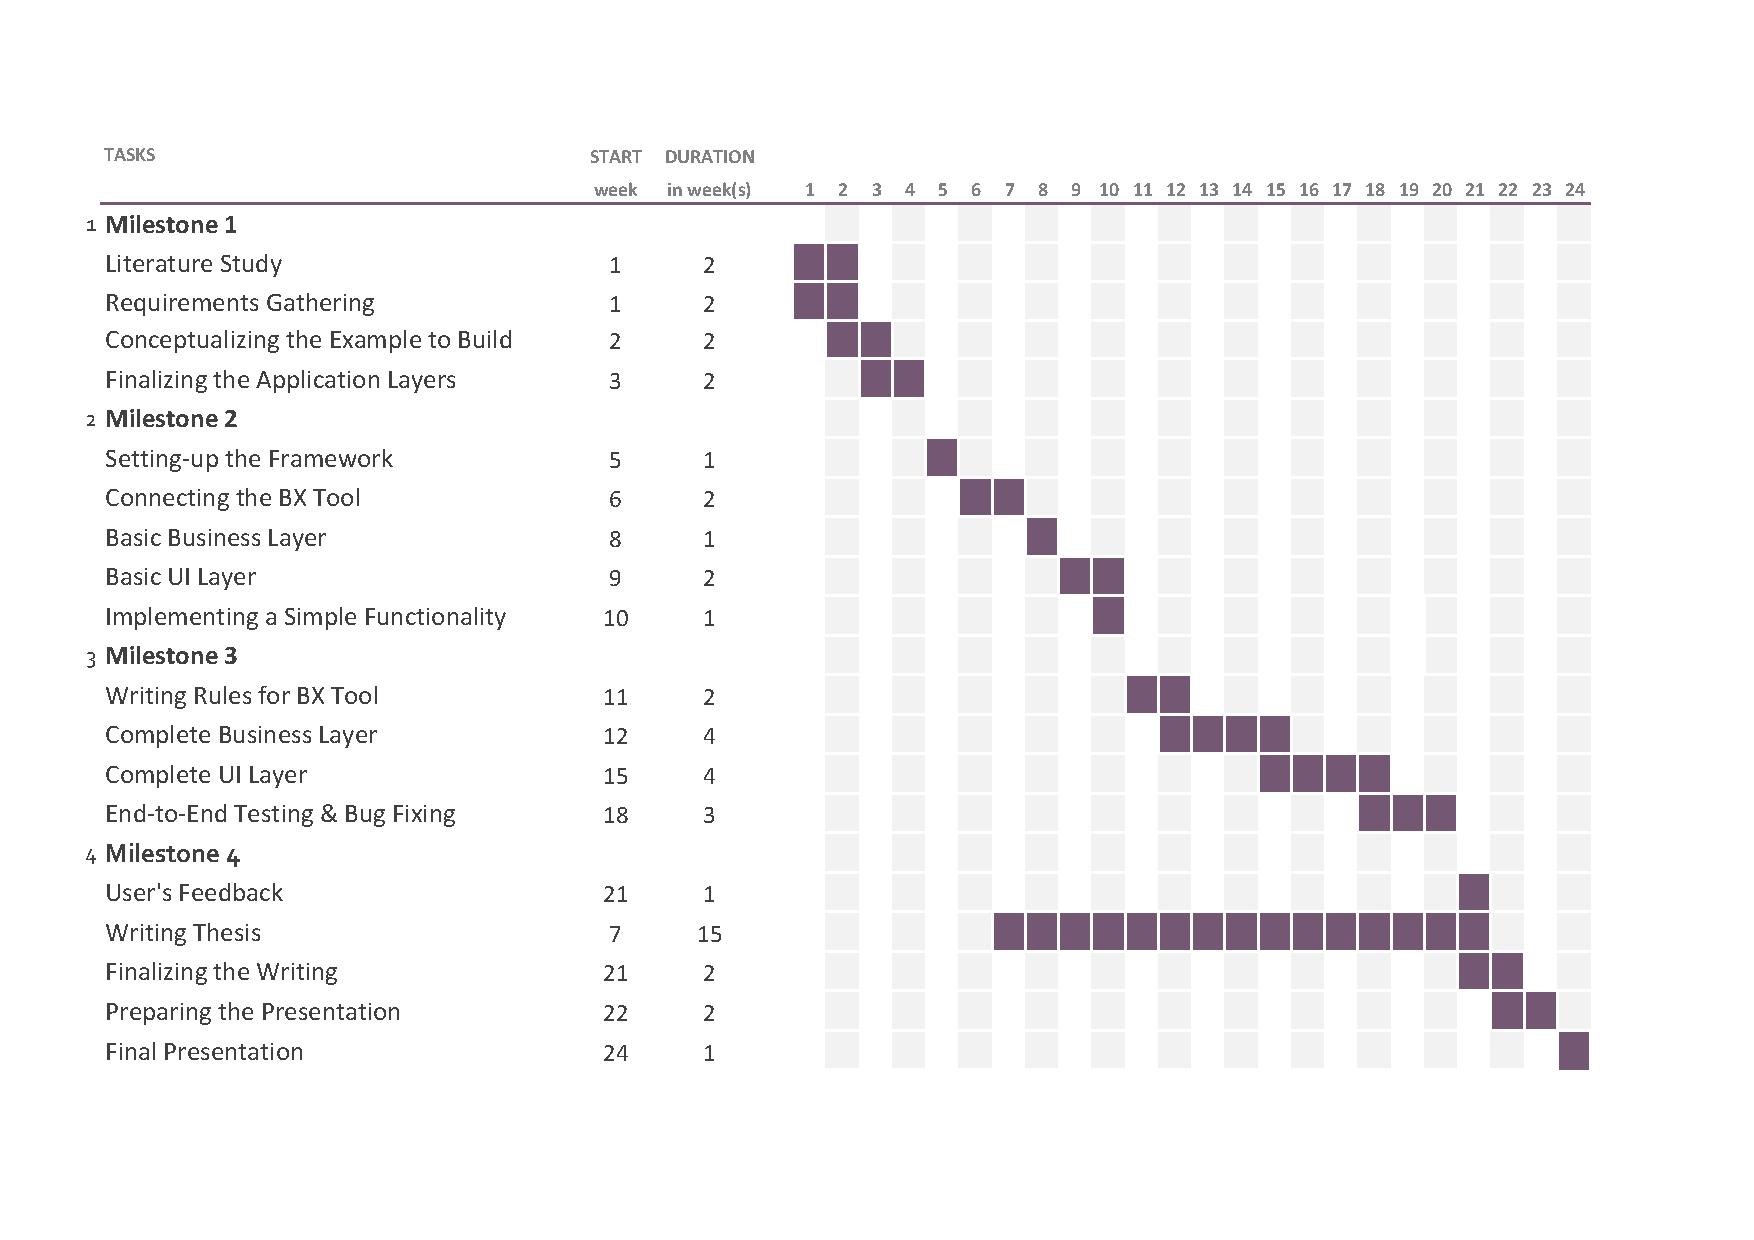
\includegraphics[width=1.1\textwidth]{figures/Time_Plan}
\captionof{figure}{Time Plan}
\label{fig:time_plan}
\end{center}

\section{Preliminary Structure of Final Documentation}\label{sec:finaldocument}
Below is the tentative structure of the document that will be available after the completion of the thesis.
\begin{enumerate}
	\item {Introduction}
	\item {Motivation}
	\item {Background and Related Work}
	\item {Research Method}
	\item {Architecture Design}
	\begin{itemize}
	    \item {High level architecture information}	
	    \item {Concrete design decision}
	    \item {UML Diagrams}
	\end{itemize}
	\item {API}
	\item {Application Walkthrough}
	\item {Outcome of Research Method: Feedback, Discussion and Learning Goals}
	\item {Future Work}
	\item {Conclusion}
\end{enumerate} 
* \textit{Above is just a preliminary and tentative structure and may vary.}

\begin{thebibliography}{1}
	
	\bibitem{bx-grace} K. Czarnecki, J. N. Foster, Z. Hu, R. L\"ammel, A. Sch\"urr, and J. F. Terwilliger,  {\em Bidirectional Transformations: A Cross-Discipline Perspective}, GRACE International Meeting , Shonan, Japan, 2008.
	
	\bibitem{bx-dagstuhl} Z. Hu, A. Sch\"urr, P. Stevens, and J. Terwilliger,  {\em Dagstuhl Seminar} \#11031 on Bidirectional Transformations "bx", Dagstuhl Reports, Vol. 1, Issue 1, pages 42-67, January 16-21 , 2011.
	
	\bibitem{bx-theoryandappl} J. Gibbons, R. F. Paige, A. Sch\"urr, J. F. Terwilliger and J. Weber, {\em Bi-directional transformations (bx) - Theory and Applications Across Disciplines}, [Online]. Available:  https://www.birs.ca/workshops/2013/13w5115/report13w5115.pdf.

	\bibitem{benchmark-BX} R. Oppermann and P. Robrecht, {\em Benchmarks for Bidirectional Transformations.} Seminar Maintaining Consistency in Model-Driven Engineering: Challenges and Techniques, University of Paderborn: Summer Term 2016.
	
	\bibitem{tgg} A. Sch\"urr. {\em Specification of graph translators with triple graph grammars.} In E. W. Mayr, G. Schmidt, and G. Tinhofer, editors, {\em Graph-Theoretic
	Concepts in Computer Science, 20th International Workshop, WG 94}, volume 903 of LNCS, pages 151-163, Herrsching, Germany, June 1994.
	
	\bibitem{bx-tgg} A. Bucaioni and R. Eramo, {\em Understanding bidirectional transformations with TGGs and JTL}, in Proc. of the Second Workshop on Bidirectional Transformations (BX 2013), no. 57, 2013.
	
	\bibitem{emoflon-part4} A. Anjorin, E. Burdon, F. Deckwerth, R. Kluge, L. Kliegel, M. Lauder, E. Leblebici, D.T\"ogel, D. Marx, L. Patzina, S. Patzina, A. Schleich, S. E. Zander, J. Reinl\"ander, and M. Wieber, {\em An Introduction to	Metamodelling and Graph Transformations with eMoflon. Part IV: Triple Graph Grammars.} [Online]. Available: 
	https://emoflon.github.io/eclipse-plugin/release/handbook/part4.pdf
    
    \bibitem{bx-community} BX Community, [Online]. Available: http://bx-community.wikidot.com/
    
    \bibitem{bx-examples} BX Community, [Online]. Available: http://bx-community.wikidot.com/examples:home
    
    \bibitem{echo} N. Macedo, T. Guimar\"aes and A. Cunha, {\em Model repair and transformation with Echo}. In Proc. ASE 2013, ACM Press, 2013.
    
    \bibitem{bigul} Hsiang-Shang Ko, Tao Zan, and Zhenjiang Hu, {\em BiGUL: A formally verified core language for putback-based bidirectional programming.} In Partial Evaluation and Program Manipulation, PEPM'16, pages 61-72. ACM, 2016.
    
    \bibitem{bigul-tutorial} Zhenjiang Hu and Hsiang-Shang Ko,  {\em Principle and Practice of Bidirectional Programming in BiGUL}, Tutorial [Online]. Available: http://www.prg.nii.ac.jp/project/bigul/tutorial.pdf
    
    \bibitem{biyacc} {\em BiYacc, tool designed to ease the work of writing parsers and printers}, [Online]. Available: http://biyacc.yozora.moe/
    
    \bibitem{share} {\em SHARE - Sharing Hosted Autonomous Research Environments}, [Online]. Available: http://is.ieis.tue.nl/staff/pvgorp/share/
    
		
\end{thebibliography}

